\documentclass{beamer}
\mode<presentation> {
%\usetheme{Madrid}
%\usetheme{default}
\usepackage{color}
\definecolor{bottomcolour}{rgb}{0.21,0.11,0.21}
\definecolor{middlecolour}{rgb}{0.21,0.11,0.21}
\setbeamercolor{structure}{fg=white}
\setbeamertemplate{frametitle}[default]%[center]
\setbeamercolor{normal text}{bg=black, fg=white}
\setbeamertemplate{background canvas}[vertical shading]
[bottom=bottomcolour, middle=middlecolour, top=black]
\setbeamertemplate{items}[circle]
\setbeamertemplate{navigation symbols}{} %no nav symbols
\setbeamercolor{block title}{use=structure,fg=white,bg=structure.fg!50!red!50!blue!100!green}
\setbeamercolor{block body}{parent=normal text,use=block title,bg=block title.bg!5!white!10!bg,fg=white}
\setbeamertemplate{navigation symbols}{}
}


\usepackage{graphicx} 
\usepackage{booktabs} 
\usepackage[utf8]{inputenc}  
\usepackage[T1]{fontenc}  
\usepackage{geometry}     
\usepackage[francais]{babel} 
\usepackage{eurosym}
\usepackage{verbatim}
\usepackage{ragged2e}
\justifying


%%%%%%%%%%%%%%%%%%%%%%%%%%%%%%%%%%%%%%%%%%%%%%%%%%%%%%%%%%%%%%%%
%% ccBeamer 0.1, 2007-07-02                                   %%
%% Written by Sebastian Pipping <webmaster@hartwork.org>      %%
%% ---------------------------------------------------------- %%
%% Licensed under Creative Commons Attribution-ShareAlike 3.0 %%
%% http://creativecommons.org/licenses/by-sa/3.0/             %%
%%%%%%%%%%%%%%%%%%%%%%%%%%%%%%%%%%%%%%%%%%%%%%%%%%%%%%%%%%%%%%%%


%% Images
\newcommand{\CcImageBy}[1]{%
	
\includegraphics[scale=#1]{creative_commons/cc_by_30.pdf}%
}
\newcommand{\CcImageCc}[1]{%
	
\includegraphics[scale=#1]{creative_commons/cc_cc_30.pdf}%
}
\newcommand{\CcImageDevNations}[1]{%
	
\includegraphics[scale=#1]{creative_commons/cc_dev_nations_30.pdf}%
}
\newcommand{\CcImageNc}[1]{%
	
\includegraphics[scale=#1]{creative_commons/cc_nc_30.pdf}%
}
\newcommand{\CcImageNd}[1]{%
	
\includegraphics[scale=#1]{creative_commons/cc_nd_30.pdf}%
}
\newcommand{\CcImagePd}[1]{%
	
\includegraphics[scale=#1]{creative_commons/cc_pd_30.pdf}%
}
\newcommand{\CcImageSa}[1]{%
	
\includegraphics[scale=#1]{creative_commons/cc_sa_30.pdf}%
}
\newcommand{\CcImageSampling}[1]{%
	
\includegraphics[scale=#1]{creative_commons/cc_sampling_30.pdf}%
}
\newcommand{\CcImageSamplingPlus}[1]{%
	
\includegraphics[scale=#1]{creative_commons/cc_sampling_plus_30.pdf}%
}


%% Groups
\newcommand{\CcGroupBy}[1]{% zoom
	\CcImageBy{#1}%
}
\newcommand{\CcGroupByNc}[2]{% zoom, gap
	\CcImageBy{#1}\hspace*{#2}\CcImageNc{#1}%
}
\newcommand{\CcGroupByNcNd}[2]{% zoom, gap
	\CcImageBy{#1}\hspace*{#2}\CcImageNc{#1}\hspace*{#2}\CcImageNd{#1}%
}
\newcommand{\CcGroupByNcSa}[2]{% zoom, gap
	\CcImageBy{#1}\hspace*{#2}\CcImageNc{#1}\hspace*{#2}\CcImageSa{#1}%
}
\newcommand{\CcGroupByNd}[2]{% zoom, gap
	\CcImageBy{#1}\hspace*{#2}\CcImageNd{#1}%
}
\newcommand{\CcGroupBySa}[2]{% zoom, gap
	\CcImageBy{#1}\hspace*{#2}\CcImageSa{#1}%
}
\newcommand{\CcGroupDevNations}[1]{% zoom
	\CcImageDevNations{#1}%
}
\newcommand{\CcGroupNcSampling}[2]{% zoom, gap
	\CcImageNc{#1}\hspace*{#2}\CcImageSampling{#1}%
}
\newcommand{\CcGroupPd}[1]{% zoom
	\CcImagePd{#1}%
}
\newcommand{\CcGroupSampling}[1]{% zoom
	\CcImageSampling{#1}%
}
\newcommand{\CcGroupSamplingPlus}[1]{% zoom
	\CcImageSamplingPlus{#1}%
}


%% Text
\newcommand{\CcLongnameBy}{Attribution}
\newcommand{\CcLongnameByNc}{Attribution-NonCommercial}
\newcommand{\CcLongnameByNcNd}{Attribution-NoDerivs}
\newcommand{\CcLongnameByNcSa}{Attribution-NonCommercial-ShareAlike}
\newcommand{\CcLongnameByNd}{Attribution-NoDerivs}
\newcommand{\CcLongnameBySa}{Attribution-ShareAlike}

\newcommand{\CcNote}[1]{% longname
	This work is licensed under the \textit{Creative Commons #1 3.0 License}.%
}


\title[Clefs PGP]{Clefs PGP} 
\author{Genma}

\begin{document}

%% Titlepage
\begin{frame}
	\titlepage
	\vfill
	\begin{center}
		\CcGroupByNcSa{0.83}{0.95ex}\\[2.5ex]
		{\tiny\CcNote{\CcLongnameByNcSa}}
		\vspace*{-2.5ex}
	\end{center}
\end{frame}


%\begin{frame}
%\frametitle{Plan} 
%\tableofcontents
%\end{frame}

%----------------------------------------------------------------------------------------
%	PRESENTATION SLIDES
%----------------------------------------------------------------------------------------


\begin{frame}
\frametitle{
\includegraphics[scale=0.4]{./Genma.jpg} \ \ \  A propos de moi  }
\begin{columns}[c] 

\column{.55\textwidth} 
\textbf{Où me trouver sur Internet?}
\begin{itemize}
\item Le Blog de Genma : http://genma.free.fr
\item Twitter : http://twitter.com/genma
\end{itemize}

\textbf{Mes centres d'intérêts?}
\\ Plein de choses dont:
\begin{itemize}
\item La veille technologique
\item Le chiffrement
\end{itemize}

\column{.5\textwidth} 
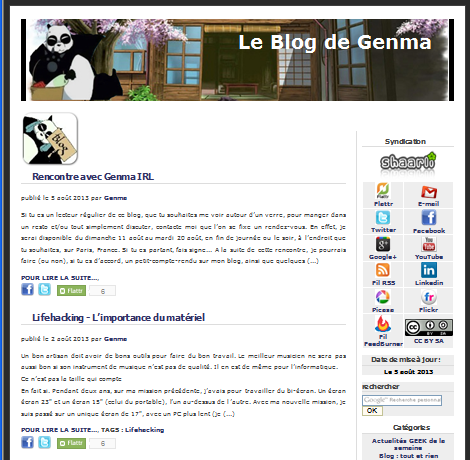
\includegraphics[width=5cm,height=5cm]{blog.png} 

\end{columns}
\end{frame}

%----------------------------------------------------------------------------------------
\begin{frame}
\begin{center}
\Huge{Qu’est ce que GPG? }
\end{center}
\end{frame}


%----------------------------------------------------------------------------------------
\begin{frame}
\frametitle{Principe de la cryptographie}
Le principe du chiffrement est de transformer à l’aide d’une clef un message clair en un message incompréhensible pour que celui qui ne dispose pas de la clef de déchiffrement. On distingue trois types d’algorithmes utilisés pour le chiffrement :
\begin{itemize}\justifying{
\item algorithmes de chiffrement simples (code de CÉSAR) ;
\item algorithmes de cryptographie symétrique fondés sur la présence d’une unique clef pour chiffrer et déchiffrer 	nécessitant autant de clef que de correspondants (AES) ;
\item algorithmes de cryptographie asymétrique fondés sur la
présence de 2 clefs, une publique (partageable) et une privée (RSA, DSA).
}
\end{itemize}
\end{frame}
%----------------------------------------------------------------------------------------

\begin{frame}
\frametitle{OpenPGP}
OpenPGP est un format de cryptographie qui définit le format
des messages, signatures ou certificats que peuvent s’envoyer
des logiciels.
\\
C’est un format pour l’échange sécurisé de données.
\end{frame}
%----------------------------------------------------------------------------------------

\begin{frame}
\frametitle{GNU Privacy Guard}
C’est une implémentation du standard OpenPGP, procédé de chiffrement à clef publique. 
\\
C’est un logiciel très stable, distribué sous la licence GNU GPL et est souvent inclus d’origine sur les systèmes d’exploitation GNU/Linux.
\end{frame}

%----------------------------------------------------------------------------------------
\begin{frame}
\begin{center}
\Huge{Générer et gérer ses clefs }
\end{center}
\end{frame}

%----------------------------------------------------------------------------------------

\begin{frame}
\frametitle{GNU Privacy Guard}
GnuPG est un système cryptographique à clef publique caractérisé par :
\begin{itemize}\justifying{
\item une clef publique, distribuée à toutes les personnes avec
qui l’utilisateur souhaite communiquer ;
\item une clef privée, gardée jalousement secrète.
}
\end{itemize}
\end{frame}
%----------------------------------------------------------------------------------------

\begin{frame}
\frametitle{Taille de la clef}
Principe :
\begin{itemize}\justifying{
\item standard entre 2048 et 4096 ;
\item plus la clef est longue, plus elle est dure à casser ;
\item plus la clef est longue, plus elle est lourde (mais chiffrement hybride) ;
\item plus la clef est longue, plus elle est longue à générer
}
\end{itemize}
\end{frame}

%----------------------------------------------------------------------------------------

\begin{frame}
\frametitle{Date d’expiration}
Validité d’une clef : temps au bout duquel les correspondants ne pourront plus utiliser cette clef pour chiffrer des données et vérifier les signatures.
\\
Comment choisir ?
\begin{itemize}\justifying{
\item 0 ou temps de vie illimité peu sécurisé : perte clef privée, vol, oubli du mot de passe,...
\item possibilité de prolongement temps de vie avant expiration
}
\end{itemize}
\end{frame}

%----------------------------------------------------------------------------------------
\begin{frame}
\frametitle{Identité de la clef}
Ce sont les informations qui apparaîtront au moment de la vérification des signatures. Attention à l’identité créée et au contexte.
\end{frame}

%----------------------------------------------------------------------------------------
\begin{frame}
\frametitle{Phrase de passe}
À bien choisir !
\begin{itemize}\justifying{
\item seule protection de la clef privée si quelqu’un possède le fichier contenant la clef privée, c’est le point faible de GnuPG ;
\item  ne devrait pas contenir de mot du dictionnaire ;
\item  devrait mélanger la casse caractères alphabétiques ;
\item devrait utiliser des caractères non alphabétiques ;
\item  taille illimitée.
}
\end{itemize}
\end{frame}


%----------------------------------------------------------------------------------------
\begin{frame}
\frametitle{Générer un certificat de révocation}

--gen-revoke génère un certificat de révocation signifiant  qu’on ne peut plus utiliser la clef publique. 2 types différents :
\begin{itemize}\justifying{
\item certificat de perte en cas d’oubli du mot de passe ou de perte de la clef ;
\item certificat de compromission si la clef privée est compromise.
}
\end{itemize}
\end{frame}

%----------------------------------------------------------------------------------------
\begin{frame}
\frametitle{Utilité}

Une bonne gestion des clefs est cruciale pour être certain que personne ne lise les messages chiffrés, en émette d’autres.
Cela permet d’être sûr de son trousseau et de garantir l’intégrité du trousseau des autres.
\end{frame}

%----------------------------------------------------------------------------------------
\begin{frame}

\frametitle{Gérer la paire de clefs}

Une clef publique est composée de :
\begin{itemize}\justifying{
\item portion publique de la clef principale de signature ;
\item  portions publiques des clefs secondaires de signature et de chiffrement ;
\item identifiants utilisés pour associer la clef à l’utilisateur (nom, commentaire optionnel, adresse mail, date de création,
date d’expiration, degré de confiance,...).
}
\end{itemize}
\end{frame}


%----------------------------------------------------------------------------------------
\begin{frame}
\frametitle{Intégrité des clefs}
La distribution des clefs publiques engendre un risque de falsification (substitution clefs, modifications identifiants utilisateurs).
\\
Pour protéger une clef publique, on utilise la partie privée de la clé principale pour signer les composantes publiques et l’identifiant utilisateur : c’est une auto-signature.
\end{frame}

%----------------------------------------------------------------------------------------
\begin{frame}
\begin{center}
\Huge{Partager les clefs }
\end{center}
\end{frame}

%----------------------------------------------------------------------------------------

\begin{frame}
\frametitle{Signer une clef}

Une clef peut être validée en vérifiant son empreinte. En la signant, on certifie qu’elle est valide via la visulaisation de son ’empreinte
\\
L’empreinte de la clef est vérifiée avec son propriétairare , on s’assure ainsi qu’on a une copie correcte de la clef. On s’assure également de l’identité de la personne que l’on a en face de soi.
\\
 Pour signer, on utilise alors la commande sign sur la clef que l’on veut éditer.
\end{frame}

%----------------------------------------------------------------------------------------

\begin{frame}
\frametitle{Confiance dans le propriétaire de la clef}

Il existe 5 niveaux de confiance pour les propriétaires de clefs :
\begin{itemize}\justifying{
\item 1 ou unknown, on ne sait rien de la façon dont la personne signe ses clefs (valeur par défaut) ;
\item  2 ou none, on sait que la personne ne vérifie pas soigneusement avant de signer ;
\item  3 ou marginal, on sait que le propriétaire a conscience de ce qu’il fait quand il signe ;
\item  4 ou full, le propriétaire sait parfaitement ce qu’il fait et une signature de lui a la même valeur que la votre ;
\item  5 ou réservé exclusivement à ses propres clefs.
}
\end{itemize}
Le niveau de confiance est une information personnelle et privée, enregistrée sur une base de donnée distincte.
\end{frame}


%----------------------------------------------------------------------------------------
\begin{frame}
\frametitle{Confiance dans le propriétaire de la clef} 
Idéalement, les clefs sont distribués personnellement. En pratique, les serveurs de clefs publiques sont utilisés pour collecter et distribuer les clefs publiques.
\\
En cas d’envoi de clef :
\begin{itemize}\justifying{
\item ajout de la clef à la base de donnée ;
\item fusion de la clef avec la clef existante si elle existe.}
\end{itemize}
En cas de requête de clef, le serveur renvoie la clef publique.
\end{frame}

%----------------------------------------------------------------------------------------
\begin{frame}
\frametitle{Distribuer ses clefs - principe des serveurs de clefs} 

Idéalement, les clefs sont distribués personnellement. En pratique, les serveurs de clefs publiques sont utilisés pour collecter et distribuer les clefs publiques.
\\
En cas d’envoi de clef :
\begin{itemize}\justifying{
\item ajout de la clef à la base de donnée ;
\item fusion de la clef avec la clef existante si elle existe.}
\end{itemize}
En cas de requête de clef, le serveur renvoie la clef publique.
\end{frame}


%----------------------------------------------------------------------------------------
\begin{frame}
\frametitle{Intérêt des serveurs de clefs} 

En cas de signature de sa clef, il faut récupérer sa clef signée et la redistribuer à tous ses contacts, pour qu’ils aient une version à jour. . .
\\
Quand quelqu’un signe une clef, il la renvoie au serveur de clef
qui rajoute la signature à sa copie de la clef publique.
\\
 Les contacts peuvent récupérer de façon autonome la clef mise à jour : le propriétaire est affranchi de la distibution.
\\
Le propriétaire récupère les signatures sur sa clef sur les serveurs.
\\
Les grands serveurs se mettent à jour les uns avec les autres, il suffit d’en sélectionner un.
\\
Il faut rafraîchir son trousseau régulièrement à cause des révocations et des expirations.
\end{frame}

%----------------------------------------------------------------------------------------
\begin{frame}
\frametitle{Importer une clef publique}
Il faut procéder en 3 étapes :
\begin{itemize}\justifying{
\item 1 trouver la clef publique souhaitée  ;
\item  2 choisir la clef de la personne que l’on cherche (et pense avoir trouver) ;
\item  3 absorber la clef}
\end{itemize}
On peut aussi avoir reçu  la clef par e-mail, de la main à la main par clef USB ou autre.
\end{frame}

%----------------------------------------------------------------------------------------
\begin{frame}
\frametitle{Id de la clef}
A une clef est associé un ID.
\end{frame}



%----------------------------------------------------------------------------------------
\begin{frame}
\begin{center}
\Huge{Utiliser ses clefs }
\end{center}
\end{frame}

%----------------------------------------------------------------------------------------
\begin{frame}
\frametitle{Principe des messages chiffrés}
Si Bob envoie un message à Alice, il le chiffre avec la clef publique d’Alice qui le déchiffrera avec sa clef privée. Et vice-versa.
\\
Pour chiffrer un message à destination de plusieurs personnes, il faut la clef publique de chacun des destinataires.
\\
Si l’on ne s’inclue pas dans les destinataires, on ne pourra pas lire son propre message.
\end{frame}

%----------------------------------------------------------------------------------------
\begin{frame}
\frametitle{Déchiffrer un message}
Pour décrypter un message, il faut la clef privée pour laquelle le message a été chiffré.
\end{frame}

%----------------------------------------------------------------------------------------
\begin{frame}
\frametitle{Signer un document}
Une signature sert à :
\begin{itemize}\justifying{
\item certifier et dater un document ;
\item permettre de vérifier que l’on est bien l’expéditeur ;
\item permettre de vérifier que le document n’a pas été modifié depuis son envoi.
}
\end{itemize}
La signature se fait avec la clef privée de l’expéditeur.
\\
Face à un document signé, on peut
\begin{itemize}\justifying{
\item vérifier la signature ;
\item extraire le document.
}
\end{itemize}
\end{frame}


%----------------------------------------------------------------------------------------
\begin{frame}
\frametitle{Protéger sa clef privée}

Essentiel :
\begin{itemize}\justifying{
\item si quelqu’un l’obtient, tout pourra être déchiffré et on peut signer en votre nom ;
\item si on la perd, on peut plus rien déchiffrer.
}
\end{itemize}
\end{frame}

%----------------------------------------------------------------------------------------
\begin{frame}
\frametitle{Protéger sa clef privée}

Il faut idéalement :
\begin{itemize}\justifying{
\item conserver le certificat de révocation et une copie de sauvegarde de la clef publique sur un support protégé en
écriture dans un lieu sûr ;
\item  conserver la clef privée sur un disque amovible protégé en écriture ;
\item  utiliser la clef privée sur une machine mono-utilisateur déconnectée du réseau ;
\item  avoir un bon mot de passe.
}
\end{itemize}
Conclusion : utiliser des sous-clefs
\end{frame}


%----------------------------------------------------------------------------------------
\begin{frame}
\frametitle{Définition des dates d’expiration}
Selon la clef, les délais d’expiration varient :
\begin{itemize}\justifying{
\item délai « long » pour la clef principale :
\item délai court pour les sous-clefs :
\item changer régulièrement est plus sécurisé (protection des
documents à venir) ;
\item en cas de perte de contrôle de la clef et de perte du
certificat de révocation.
}
\end{itemize}
\end{frame}


%----------------------------------------------------------------------------------------
\begin{frame}
\frametitle{Utilisation des clefs secondaires}

Les consignes sont :
\begin{itemize}\justifying{
\item changer régulièrement afin de protéger les documents chiffrés ultérieurement ;
\item publier la nouvelle clef avant l’expiration de la précédente ;
\item faire valider sa clef principale par ses correspondants ;
\item aucun intérêt à avoir plusieurs clefs secondaires de
\item chiffrement actives à un temps donné ;
\item aucun problème à avoir plusieurs clefs secondaires expirées dans une paire de clef donnée.
}
\end{itemize}
\end{frame}

%----------------------------------------------------------------------------------------
\begin{frame}
\frametitle{Gérer sa toile de confiance}

Il faut garder en tête que l’appartenance au réseau de confiance n’est pas une garantie de bonne foi, c’est un indice de validité de l’identité de la personne.
 \\
Ce qui compte, ce n’est pas le nombre de signatures, mais la
qualité des signatures.
 \\
Il existe deux façons de gérer sa confiance :
\begin{itemize}\justifying{
\item modèle PGP ou la validité d’acquière par 1 confiance totale ou 3 confiances marginales ;
\item  modèle personnalisé en fonction de l’usage des indices de confiances.
}
\end{itemize}
\end{frame}

%----------------------------------------------------------------------------------------
\begin{frame}
\frametitle{Faire de la propagande !}
\begin{itemize}\justifying{
\item commencer avec les personnes avec qui vous avez appris ;
\item introduiser subtilement une signature et répondre aux interrogations soulevées par la mystérieuse pièce-jointe ;
\item aller à des key-signing parties !
}
\end{itemize}
\end{frame}


%----------------------------------------------------------------------------------------
\begin{frame}
\begin{center}
\Huge{Questions - Démonstration }
\end{center}
\end{frame}

%----------------------------------------------------------------------------------------
\begin{frame}
\begin{center}
\Huge{ANNEXES }
\end{center}
\end{frame}

%----------------------------------------------------------------------------------------
\begin{frame}

\frametitle{Ajouter des composantes à une clef}
On peut vouloir ajouter différentes composantes :

\begin{itemize}\justifying{
\item identifiants utilisateurs avec adduid en cas de multiples identités ;
\item sous-clefs avec addkey car changer de clef principale nécessite de refaire les certifications, et il est recommandé
de changer de sous-clefs régulièrement (3 ans) et d’utiliser des sous-clefs différentes sur des machines différentes.
}
\end{itemize}
\end{frame}

%----------------------------------------------------------------------------------------
\begin{frame}

\frametitle{Retirer des composantes à une clef}

Les sous-clefs et les identifiants utilisateurs peuvent être effacés :
\begin{itemize}\justifying{
\item 
sélection de l’item à effacer par les sélecteurs key et uid (key 2 sélectionne la seconde sous-clef) ;
\item  effacement de l’item sélectionné par delkey ou deluid.
}
\end{itemize}
L’effacement complique la distibution des clefs. Lors de l’import ou de l’envoi sur un serveur de la clef publique, la fusion
restaure les éléments effacés.
\end{frame}


%----------------------------------------------------------------------------------------
\begin{frame}

\frametitle{Révoquer les composantes d’une clef}
\begin{itemize}\justifying{
\item pour une sous-clef, on utilise revkey après avoir sélectionné la sous-clef (auto-signature de révocation) ;
\item pour une signature, on utilise revsig, l’interface révoquée ;
\item pour un identifiant utilisateur, on révoque son auto-signature.
\item 
}
\end{itemize}
La révocation est toujours visible lors distribution et màj de la clef publique. Cela garantit que les autres aient une version
intègre de la clef.

\end{frame}


%----------------------------------------------------------------------------------------
%--\begin{frame}

%--\frametitle{Mettre à jour la date d’expiration de la clef}
%--\begin{itemize}\justifying{
%--\item 
%--\item 
%--}
%--\end{itemize}
%--\end{frame}

\end{document}
